\chapter{Programmbeschreibung}\label{ch:programmbeschreibung}
\newcommand{\fakesection}[1]{%
    \par\refstepcounter{section}% Increase section counter
    \sectionmark{#1}% Add section mark (header)
    \addcontentsline{toc}{section}{\protect\numberline{\thesection}#1}% Add section to ToC
}
\newcommand{\fakesubsection}[1]{%
    \par\refstepcounter{subsection}% Increase subsection counter
    \subsectionmark{#1}% Add subsection mark (header)
    \addcontentsline{toc}{subsection}{\protect\numberline{\thesubsection}#1}% Add subsection to ToC
}

\fakesection{Klassendiagramm}\label{sec:klassendiagramm}
\begin{center}
    \makebox[\textwidth]{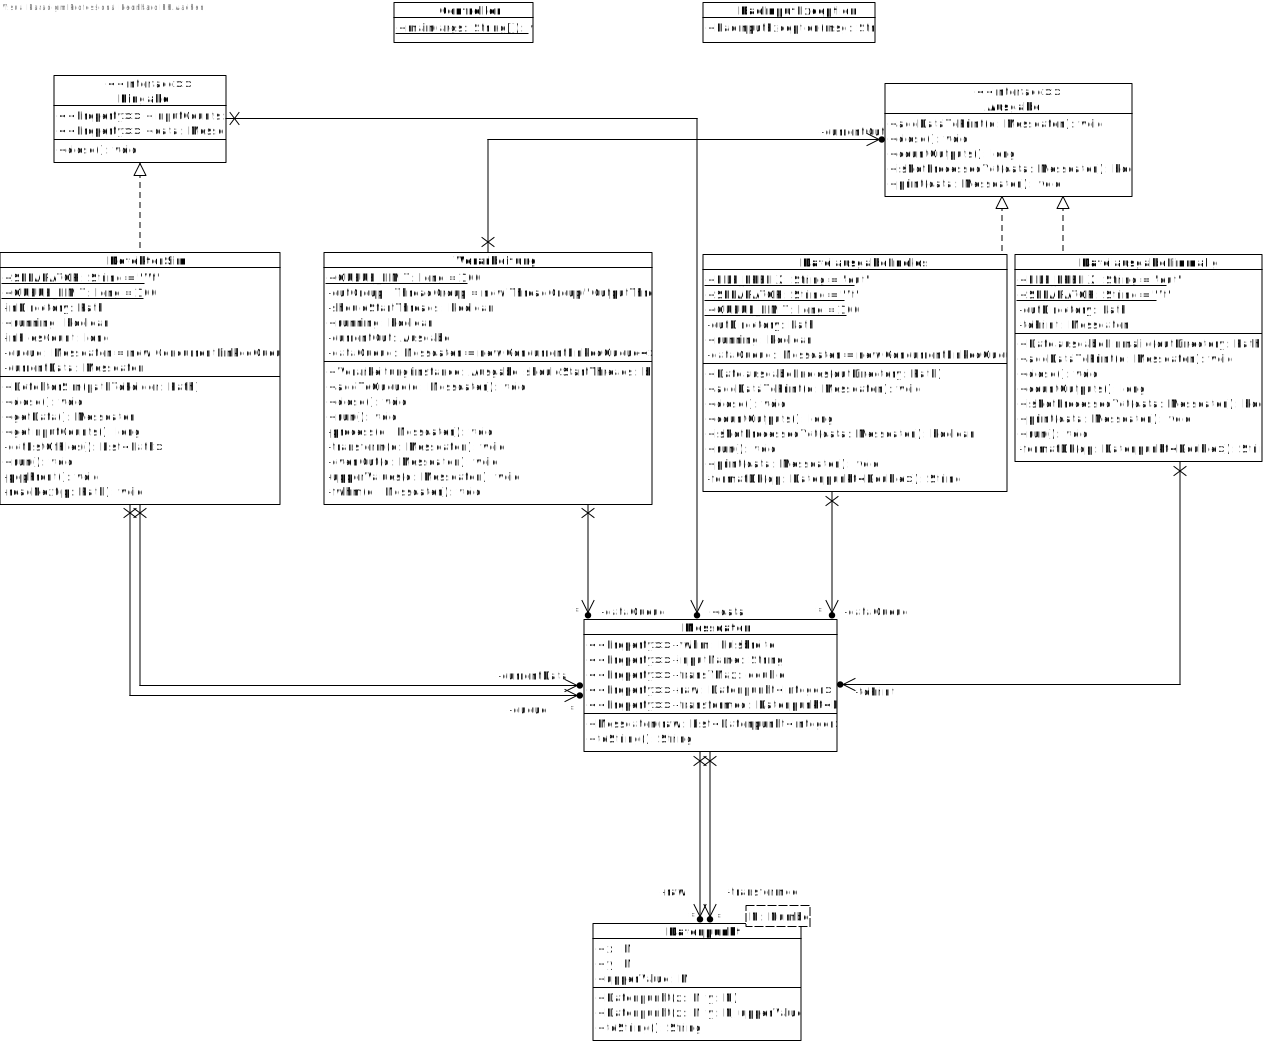
\includegraphics[width=\paperwidth]{images/Class Diagram1}}
\end{center}

\fakesection{Struktogramme}\label{sec:structogram}
\fakesubsection{Controller.main()}\label{subsec:controller_main}
\begin{center}
    \makebox[\textwidth]{\includesvg[width=\textwidth]{images/Controller_main}}
\end{center}
\fakesubsection{Verarbeitung.transform()}\label{subsec:verarbeitung_transform}
\begin{center}
    \makebox[\textwidth]{\includesvg[width=\textwidth]{images/Verarbeitung_transform}}
\end{center}
\fakesubsection{Verarbeitung.evenOut()}\label{subsec:verarbeitung_evenOut}
\begin{center}
    \makebox[\textwidth]{\includesvg[width=\textwidth]{images/Verarbeitung_evenOut}}
\end{center}
\fakesubsection{Verarbeitung.upperValues()}\label{subsec:verarbeitung_uppverValues}
\begin{center}
    \makebox[\textwidth]{\includesvg[height=\textheight]{images/Verarbeitung_upperValues}}
\end{center}
\fakesubsection{Verarbeitung.fwhm}\label{subsec:verarbeitung_fwhm}
\begin{center}
    \makebox[\textwidth]{\includesvg[width=\textwidth]{images/Verarbeitung_fwhm}}
\end{center}


\fakesection{Sequenzdiagramm}\label{sec:sequenzdiagramm}
\includesvg[width=\textwidth]{images/sequenz}


\section{Entwicklungsdokumentation}\label{sec:entwicklerdokumentation}
Die Dokumentation des Programms wurde in Javadoc vorgenommen und kann im Ordner javadoc eingesehen werden.
Hierzu kann die index.html aufgerufen werden.